
%
%  $Description: Author guidelines and sample document in LaTeX 2.09$ 
%
%  $Author: ienne $
%  $Date: 1995/09/15 15:20:59 $
%  $Revision: 1.4 $
%

\documentclass[times, 10pt,twocolumn]{article} 
\usepackage{latex8}
\usepackage{times}
\usepackage{graphicx}
\usepackage{epstopdf}
\usepackage{enumitem}
\usepackage[font=small]{caption}
\usepackage[utf8]{inputenc}
\usepackage{subcaption}

%\documentstyle[times,art10,twocolumn,latex8]{article}

%------------------------------------------------------------------------- 
% take the % away on next line to produce the final camera-ready version 
\pagestyle{empty}

%------------------------------------------------------------------------- 
\begin{document}

\title{Distributed Software Transactional Memory}

\maketitle
\thispagestyle{empty}

\begin{abstract}
   The present report describes the implementation details of a fault-tolerant,
   replicated, distributed software transactional memory. Performance of protocol is
   evaluated through latency and bandwidth required, overall throughput, load balancing
   of data storage and processing.
   Furthermore, a critical assessment of the quality of the protocol and future work is 
   also provided. 
\end{abstract}

%------------------------------------------------------------------------- 
\Section{Introduction}
Due to the cloud computing revolution in computing, 
today’s world has increasingly moved to cloud-based services rather than maintaining their 
own infrastructure. The cloud service providers are well equipped with the hardware and
 software infrastructure to provide better services by applying concepts of {\it Distributed Computing}. 

In this model of computing, one of the main problems that providers face is concurrent transactions;
 how the system behaves when multiple users access/manipulate an object at the same time; how to maintain 
the proper order of commit and how to resolve conflicting operations. 
The paper describes the solution for handling transactions in a replicated, fault-tolernt, distributed system. 

Section \ref{sec:arch} introduces an overview of each scenario. Section 
\ref{sec:algor} discusses the algorithms used for concurrency control, 
transaction management and Client-Server communication


%------------------------------------------------------------------------- 
\Section{Architecture}
\label{sec:arch}

The assumption made for all the sections below is that the Master is a perfect process. 
The names Object Servers and Servers are used interchangeably and refer to any non-Master and non-Client process
 that participates in a transaction.
The Master also acts as the{\it Coordinator} for handling transactions and{\it Replica Manager} for eagerly replicating
objects among the Object Servers. The main assumption is that the Master does not fail, only Object Servers do.

Subsection \ref{subsec:repl} details the replication steps when a commit occurs, 
Subsection \ref{subsec:grmemb} lists the details of redistribution of objects among servers after a server fail or join. 
Further details on the reponsibilities of the Coordinator/Master are in Subsection \ref{subsec:respon}.
%------------------------------------------------------------------------- 
\SubSection{Replication}
\label{subsec:repl}
Information such as IP address and port number of the Server is stored by the Master which, then, issues unique identifiers for each Server. 
Once the Object Server has been issued an identifier and notified the Master of joining the group of available servers, 
it can be connected by Clients for handling transactions. Transaction identifiers (TID) should be unique to the whole system 
therefore the Master server will keep track of the global sequence of TIDs.

When the Coordinator receives a \texttt{Commit} call along with the Transaction ID,
 and the list of UIDs, it will update each workers' replica. Once the replication is completed,
 the Coordinator returns from the transaction and notifies the client of the commit's result.

%------------------------------------------------------------------------- 
\SubSection{Group Membership Change/Stabilization}
\label{subsec:grmemb}
Since the Master server also assumes the role of a failure detector,
 upon observing a node failure, it updates its list of available workers
 and sends it to the workers. The{\it Coordinator} calls the \texttt{Stabilizer()},
 which monitors existing transactions and makes sure that they finalize.

The following steps are taken once failure is detected: 
\begin{enumerate}
\item the Coordinator no longer issues TIDs for upcoming requests
\item the Coordinator commits or aborts the existing, in-flight, transactions
\item the replica server names list along with the group view (or server list) is updated, 
then sent to servers
\item \texttt{Shuffle()} is executed to redistribute its allotted objects and the respective replica objects 
\item misplaced (now outdated) replica objects are cleared
\item upon the completion of all the above steps, once there is a stable group membership, 
the Coordinator will be issuing new TIDs
\end{enumerate}

The pending, in-flight transactions, are given a few seconds in order to commit. 
Once the the timeout period has passed, the Coordinator aborts the pending transactions in order to 
stabilize the system.

%------------------------------------------------------------------------- 
\SubSection{Coordinator/Master responsiblities}
\label{subsec:respon}
% merged the coordinator and master sections here
The Master server's responsibilities, from bootstrapping the servers to detecting failures and joins,
 plays an central role in the architecture and is the backbone for handling transactions.
As a failure detector, the Master server receives periodic heartbeat timestamps from servers, stores them and, periodically,
 checks the difference between the last timestamp and current time to determine whether a server has failed.

As the Coordinator, it issues TIDs for all the clients. The TID is the current date and time converted into ticks, resulting in a 
(long) value. To assure unicity, even if the generation of TIDs generation code is synchronized, the thread
issuing TIDs will also sleep for one millisecond. Thus, avoiding any possibility of issuing the same TID to different clients.
The issued TIDs are being tracked in order to monitor the current active transactions of the whole system. 
Once a transaction aborts or commits the TIDs are no longer tracked/removed. 

Once a server failure has been detected, the{\it stabilisation} of objects begins - as detailed in
Section \cite{subsec:grmemb}.

\SubSection{Object Server}
\label{subsec:objserv}
The Object Servers are the location of PadInt objects. This objects held in different servers
are manipulated by different clients via different read/write operation requests issued by 
different clients.

The timestamp ordering prevents deadlocks among transaction, but there is a chance to have
long waits if a certain client begins a transaction, processes different requests but does not 
commit. To prevent other clients from waiting, a periodic inspection on the tentative writes to calculate
its lifespan in the tentative list is used. Assuming that a certain transaction should not exceed
a certain time period, we included a timeout so that it will abort that long running transaction. 

Furthermore, \texttt{Freeze} and \texttt{Fail} functions were also implemented to test the system verifiable with different use cases. 
For the implementation of \texttt{Freeze}, we did a trick which solved lot of synchronization issues, by
 making use of \texttt{Monitors.Wait}. Once a server has been issued a read/write by the client, 
the server will execute the operation as normal, but instead of returning, it waits. 
To wake up all the operations issued by the client, the client can use the \texttt{recover}.
The implementation of \texttt{Fail} consists in having the server no longer sending heartbeats to the Master.
Thus, the Master server, upon its periodic timestamp difference check will identify the failed server.
 

\SubSection{Client}
\label{subsec:client}
Through this proxy for the actual client application accesses the PadInt objects stored in the servers. 
Its exposed API meets the specification requirements and are necessary in order to 
successfully complete a transaction. 
 
It asks the Coordinator for the TID and loads the latest (Object Server) View from the Master,
 if it identified that the View has been changed.

The view change is detected by appending the current view's timestamp at the end of eached retrieved TID. 
The Client stores each retrieved views' timestamp and compares it with the one attached to a newly issued TID. 
If they're different, it loads the new, latest, (Object Server) view (or map, or list) from the Master. 

The newly updated server map is used for deciding which of the worker servers should hold which PadInt created 
by the client application. 
Moreover, this component keeps track of the UIDs accessed by a certain transaction and pass this list along
 with the transaction commit/abort requests, so that the coordinator can only consult the relevant object servers
 without probing every server.


%------------------------------------------------------------------------- 
\Section{Algorithms}
\label{sec:algor}
%------------------------------------------------------------------------ 
\SubSection{Communication}
The sequence diagram, in Figure \ref{fig:seqd}, depicts the communication between the client, coordinator and object servers,
assuming no failures or joins - any group membership change. 

\begin{figure*}
\centering
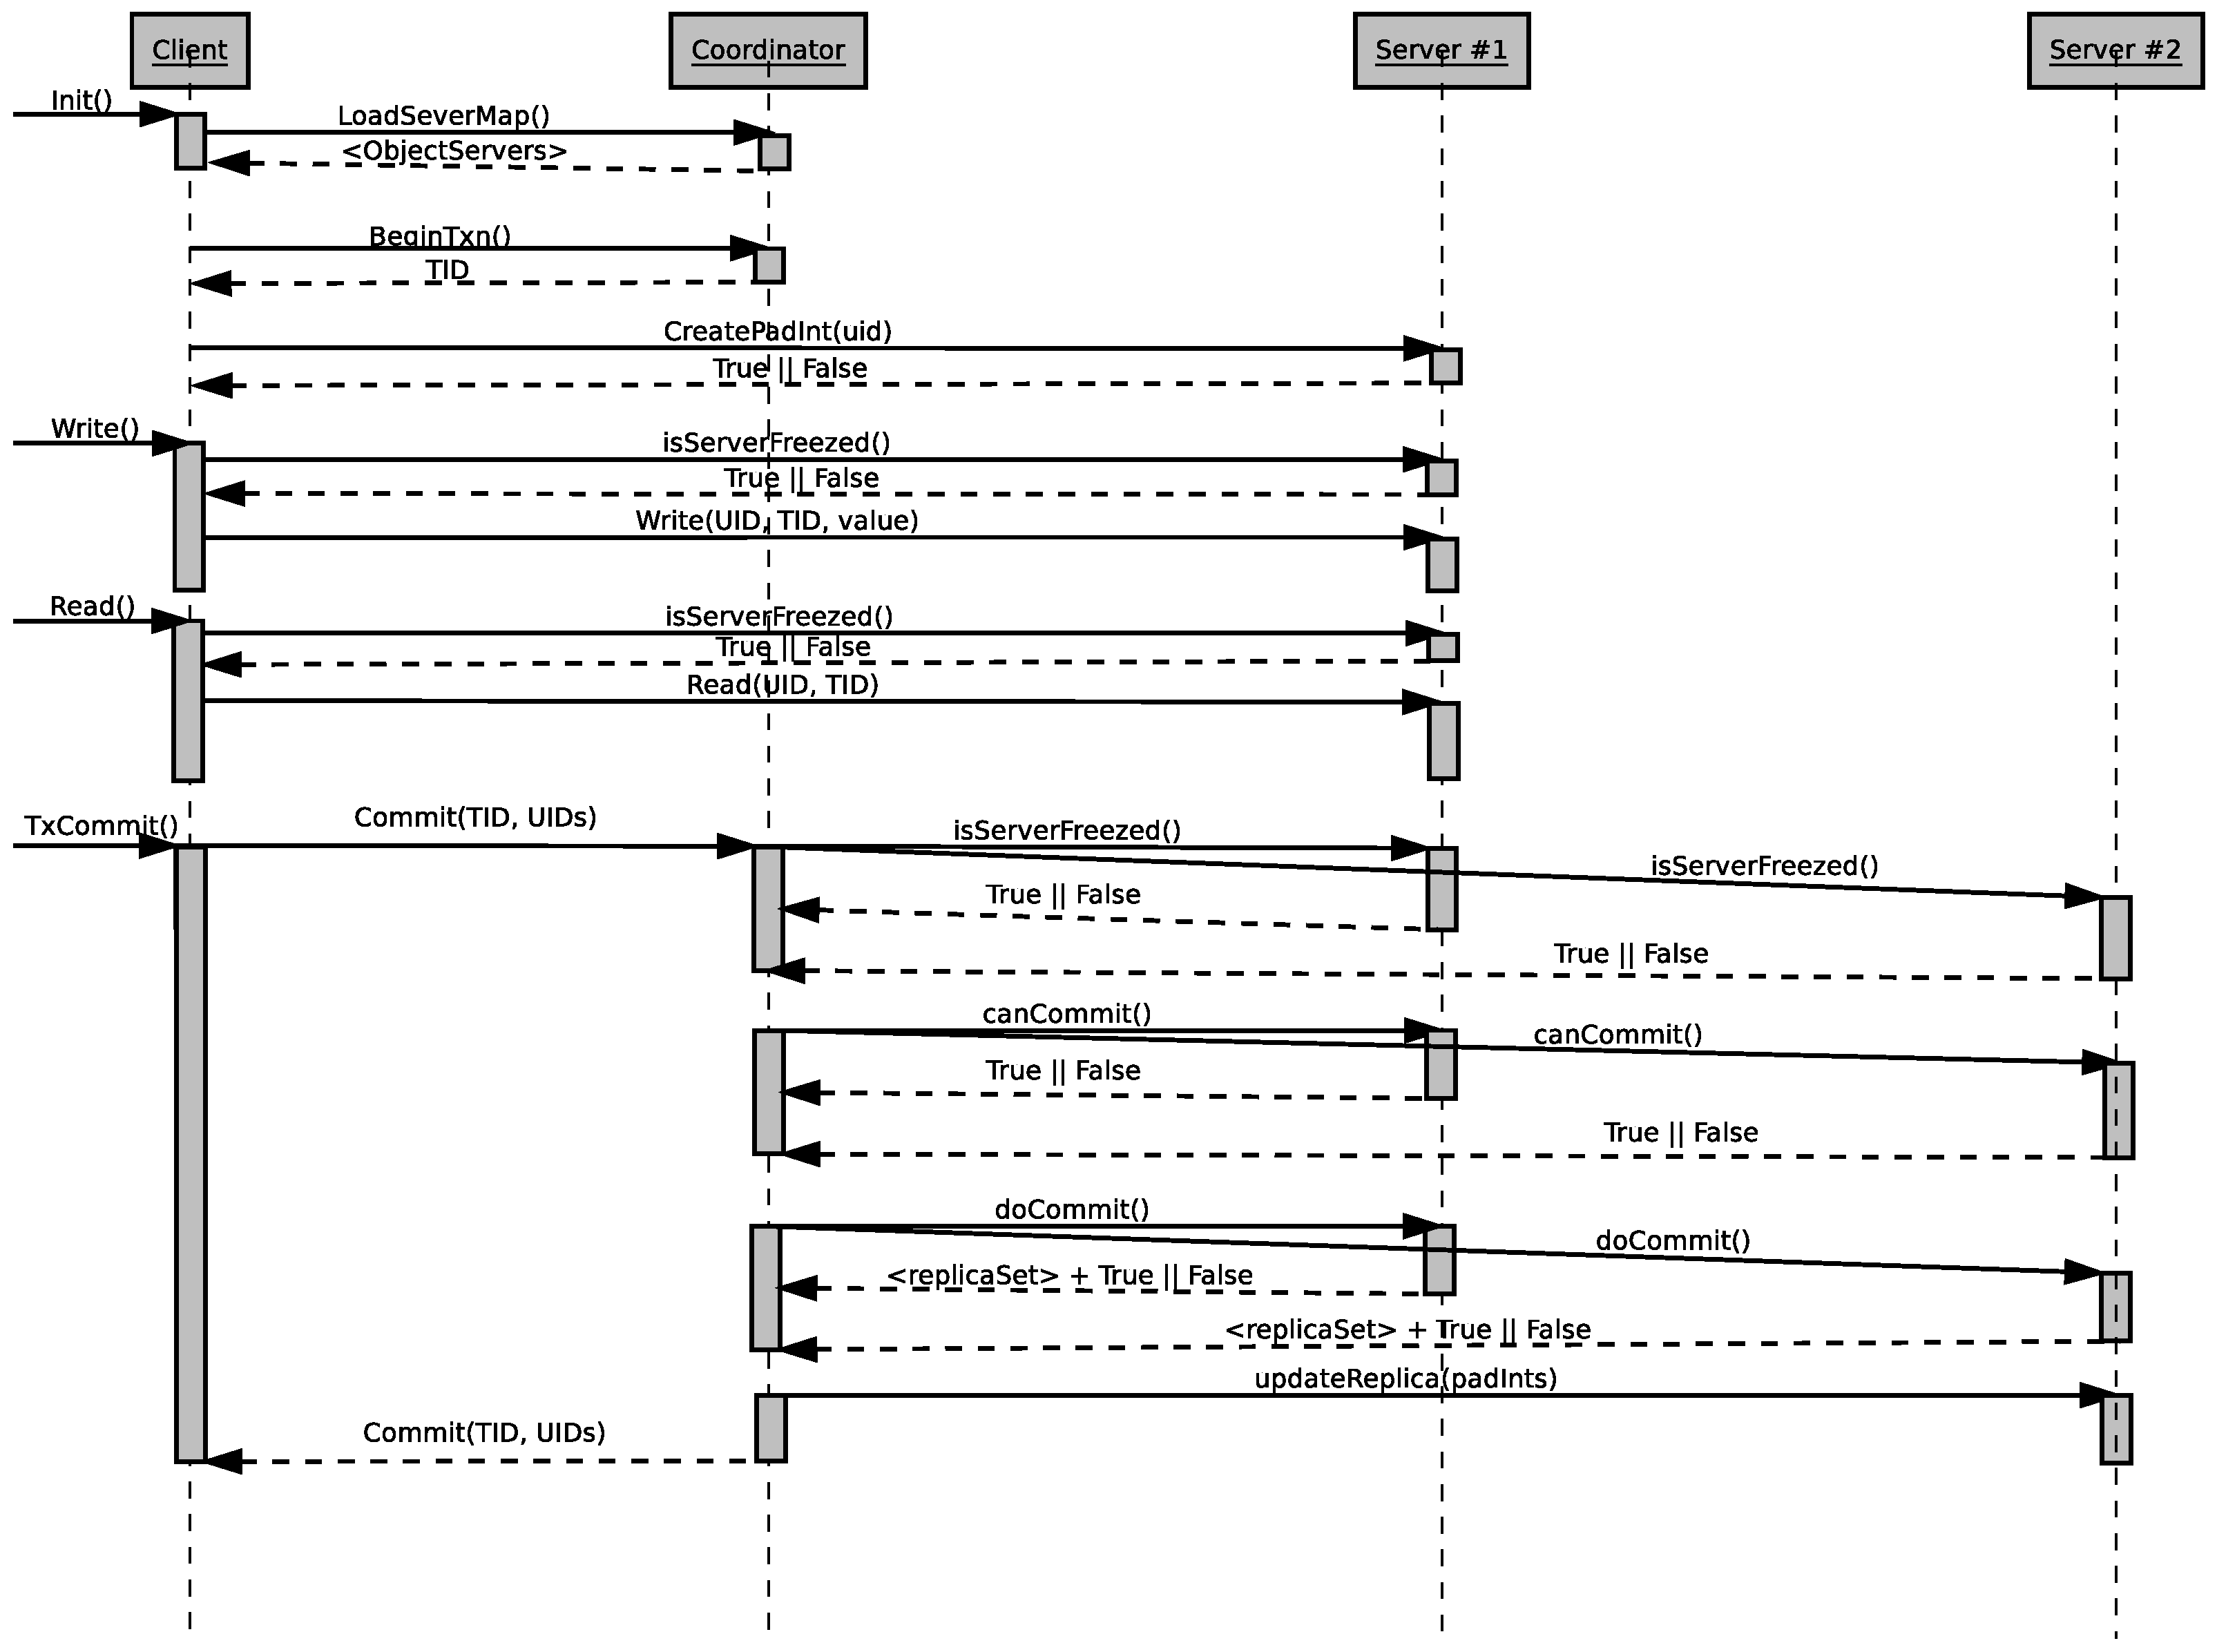
\includegraphics[scale=0.25]{seqDiaCommSteps.eps}
\caption{Communication between the client, coordinator and servers during a transaction}
\label{fig:seqd}
\end{figure*}

%------------------------------------------------------------------------- 
\SubSection{Transaction Management and Concurrency Control}
\label{subsec:transmgt}
The {\it Flat Transaction} model allows for a client to manipulate objects on multiple servers in a single transaction. With regards to concurrency control, {\it Timestamp Ordering} will be used for this project. 

The advantages of choosing {\it Timestamp Ordering} over {\it Two-Phase Locking} or {\it Optimistic Concurrency} options are the following: 
\begin{itemize}[noitemsep, nolistsep]
\item Deadlock prevention - common with the use of locks
\item Better performance for transactions with predominantly {\it read} operations \cite{bernstein1987concurrency}
\item Faster conflict resolution when compared to locking - transactions are aborted immediately.
\end{itemize}

Figure \ref{fig:seqd} illustrates the steps between the Client, Coordinator and Object Serves during a transaction, 
with {\it write} and {\it read} operations, followed by a commit. Once a commit request is received, it will follow 
the two-phase commit protocol and, in addition, it will contact the replica manager to replicate the latest commit
value returned at the end of the two phase commit. Once replication is completed the result of the commit({\bf True}
or {\bf False}) is returned. Thus, the replication model is {\it Eager primary backup}. 

%-------------------------------------------------------------------------
\SubSection{Timestamp Ordering and Deadlock Detection}
\label{subsec:dldetect}
Due to the use of timestamp ordering for concurrency control, there is limited probability of deadlock occurance.
Each transaction is assigned a unique timestamp on start. Each operation in a transaction is validated when it is carried out.
Should a transaction fail the validation it is immediately aborted, but can be restarted by the Client. The Client is issued with a globally unique transaction timestamp by the Coordinator. The servers are jointly responsible for ensuring serial equivalence. For instance, server S1 access an object before S2, thus server S1 appears before S2 for all objects. The Coordinators must agree on timestamp ordering to maintain all servers synchronised with the same ordering. The timestamp consists of a {\it (local timestamp, server-id)} pair and is kept synchronized by the use of local physical clocks coordinated by the Master.

Conflict resolution is performed at each operation.
The basic timestamp ordering rule is based on operation conflicts and is very simple:
{\it A transaction’s request to write an object is valid only if that object was last read and written by earlier transactions. A transaction’s request to read an object is valid only if that object was
last written by an earlier transaction.}\cite{coulouris2005distributed}. Each transaction has its own tentative version of each object it accesses, such that multiple concurrent transactions can access the same object. The tentative versions of each object are committed in the order determined by the timestamps of their transactions by transactions waiting, if necessary, for earlier transactions to complete their writes.
Since transactions only wait for earlier ones (thus, no cycle occurs in the wait-for graph), no deadlocks occur.

Conflict resolution is performed at each operation. If the resolution is to abort the transaction the Coordinator is informed and it will abort the transaction for all the participants.
Finally, we integrated the above implemented components in order to achieve the fault-tolerant, 
replicated, and distributed software transactional memory.


\Section{Evaluation}

\begin{figure}
\centering
\includegraphics[scale=0.4]{withonefailure.eps}
\caption{Out of 600 transactions, 200 by each server, normalized results of 3 simulations}
\label{fig:onef}
\end{figure}


\begin{figure}
\centering
\includegraphics[scale=0.4]{nofailures.eps}
\caption{Out of 600 transactions, 200 by each server, normalized results of 3 simulations}
\label{fig:noff}
\end{figure}


%------------------------------------------------------------------------- 
\Section{Conclusion}
Across the sections we discussed the solutions proposed in order to implement Distributed Software Transactional Memory System.
Our solution addresses two scenarios: perfect links and processes and a fault tolerant system.
A very important goal has been to provide a simple solution which would eliminate conflicts in transactions without encountering the inefficiency of a distributed environment. 
The sections and subsections address each of the two architectures individually in order to provide a clearer distinction of responsibilities and complexity of the system.
Furthermore,{\it Timestamp Ordering} based concurrency control aids in eliminating local and global deadlocks which represents one of the major issues that need to be addressed in DSTMs.

Finally, we believe that the concepts we came across in the discussion of this paper builds a firm foundation for implementing this solution in an efficient manner.
%------------------------------------------------------------------------- 
%- \Section{References}

\bibliographystyle{latex8}
\bibliography{latex8}

%------------------------------------------------------------------------- 
\end{document}
